
\section{CPU vs GPU Comparison}
\subsection{Device Characteristics}
The two devices being used are both examples of high-end consumer hardware, suited for hobbyist high performance applications. Table~\ref{tab:devchars} shows the different characteristics of both devices.

\begin{table}[h]
\centering
\resizebox{\columnwidth}{!}{%
\begin{tabular}{l  l  l}
\hline
\textbf{Device Characteristic} & \textbf{Intel Device} & \textbf{NVIDIA Device} \\
\hline
Device name:                 & Intel(R) Xeon(R) CPU E5-2686 v4 & Tesla K80 \\
Global memory (MB):          & 61406 								 & 11439  \\
Local memory (KB):           & 32 									 & 48\\
Max. compute units:          & 4 										 & 13\\
Max. work groups:            & 8192 									 & 1024\\
Max. work items:             & [8192, 8192, 8192] 						 & [1024, 1024, 64] \\
Max. memory allocation (bytes): & 16097245184 							     & 2998894592 \\ 
Max. clock frequency (MHz):        & 2300 									 & 823\\
\hline
\end{tabular}
}
\caption{Comparison of device characteristics}
\label{tab:devchars}

\end{table}




\subsection{Sum kernel performance}
Table~\ref{tab:kernel} shows the results of running the sum kernel on both CPU and GPU, on a variety of different vector sizes. Each program was run twice, to eliminate variance from caching. Vectors of up to 10\textsuperscript{7} elements were run successfully. Trying with 10\textsuperscript{8} elements failed to run, as the memory buffers on either device did not have the requisite cache size for storage. An implementation could be made where elements are swapped in and out of device memory to allow for 10\textsuperscript{8} elements to be processed, but that would introduce speed differences due to memory operations and would be outside the scope of this task. 



\begin{table}[h]
\centering
\resizebox{\columnwidth}{!}{%
\begin{tabular}{l  c  c c}
\hline
\textbf{Vector Size} & \textbf{CPU Time [ms]} & \textbf{GPU Time [ms]} &\textbf{CPU/GPU speed-up}\\
\hline
1e2 (run 1) & 1.81 & 1.55 &  1.168 \\
1e2 (run 2) & 1.81 & 1.55 &  1.168 \\
1e4 (run 1) & 1.89 & 1.59 &  1.189 \\
1e4 (run 2) & 1.89 & 1.59 &  1.189 \\
1e6 (run 1) & 3.60 & 3.43 &  1.050 \\
1e6 (run 2) & 3.60 & 3.42 &  1.053 \\
1e7 (run 1) & 55.2 & 16.4 &  3.367 \\
1e7 (run 2) & 54.8 & 16.4 &  3.341 \\
1e8 (run 1) & 476  & 146  &  3.260 \\
1e8 (run 2) & 475  & 146  &  3.253 \\

\hline
\end{tabular}
}
\caption{CPU vs GPU performance on sum kernel}
\label{tab:kernel}

\end{table}







\subsection{Factor count performance}

Table~\ref{tab:factors} shows the results of running the factor count program on both CPU and GPU, on a variety of different matrix sizes. The golden measure (GM) was performed sequentially using Python code on the system's Intel CPU. This gives a realistic comparison to the parallel devices of the system, rather than comparing it with the performance of an unrelated machine, in a different hardware/software environment. The golden measure took too long to complete on datasets larger than 10,000 elements. The factor count program is a coarse parallel operation, requiring no communication between threads. It has more computation per thread than the sum kernel, which helps to explain the difference in speed-up between the two programs.

\begin{table}[h]
\centering
\resizebox{\columnwidth}{!}{%
\begin{tabular}{l  c  c c}
\hline
\textbf{Matrix Size} & \textbf{CPU Time [ms]} & \textbf{GPU Time [ms]} &\textbf{CPU/GPU speed-up}\\
\hline
1e2 (GM) & 17.9 & - & - \\
1e4 (GM) & 1800 & - & - \\
1e2 (run 1) & 2.08 & 1.55 & 1.342  \\
1e2 (run 2) & 2.07 & 1.54 & 1.344 \\
1e4 (run 1) & 2.46 & 1.57 & 1.567 \\
1e4 (run 2) & 2.47 & 1.58 & 1.563 \\
1e6 (run 1) & 61.5 & 4.35 & 14.14 \\
1e6 (run 2) & 61.5 & 4.35 & 14.14 \\
1e8 (run 1) & 5980 & 283  & 21.13 \\
1e8 (run 2) & 5980 & 284  & 21.06 \\

\hline
\end{tabular}
}
\caption{CPU vs GPU performance counting factors}
\label{tab:factors}

\end{table}


\subsection{Average Speed-up}
Analysis of the results shows that the different tasks were both favoured by the GPU as the number of elements increased. Figure~\ref{fig:speedup} demonstrates that the sum program yielded less speed-up, and had only began to show improvement between 10\textsuperscript{6} and 10\textsuperscript{7} elements. The average speed-up of the GPU versus the CPU implementation was 2.0038; almost exactly double. The factor count program began to show improvements earlier, and continued to increase until the limits of the devices' memory was reached. Its average speed-up was 9.536 over all cases, but this is somewhat misleading, given the large discrepancy between small and large vector sizes.


\begin{figure}[h]
\centering
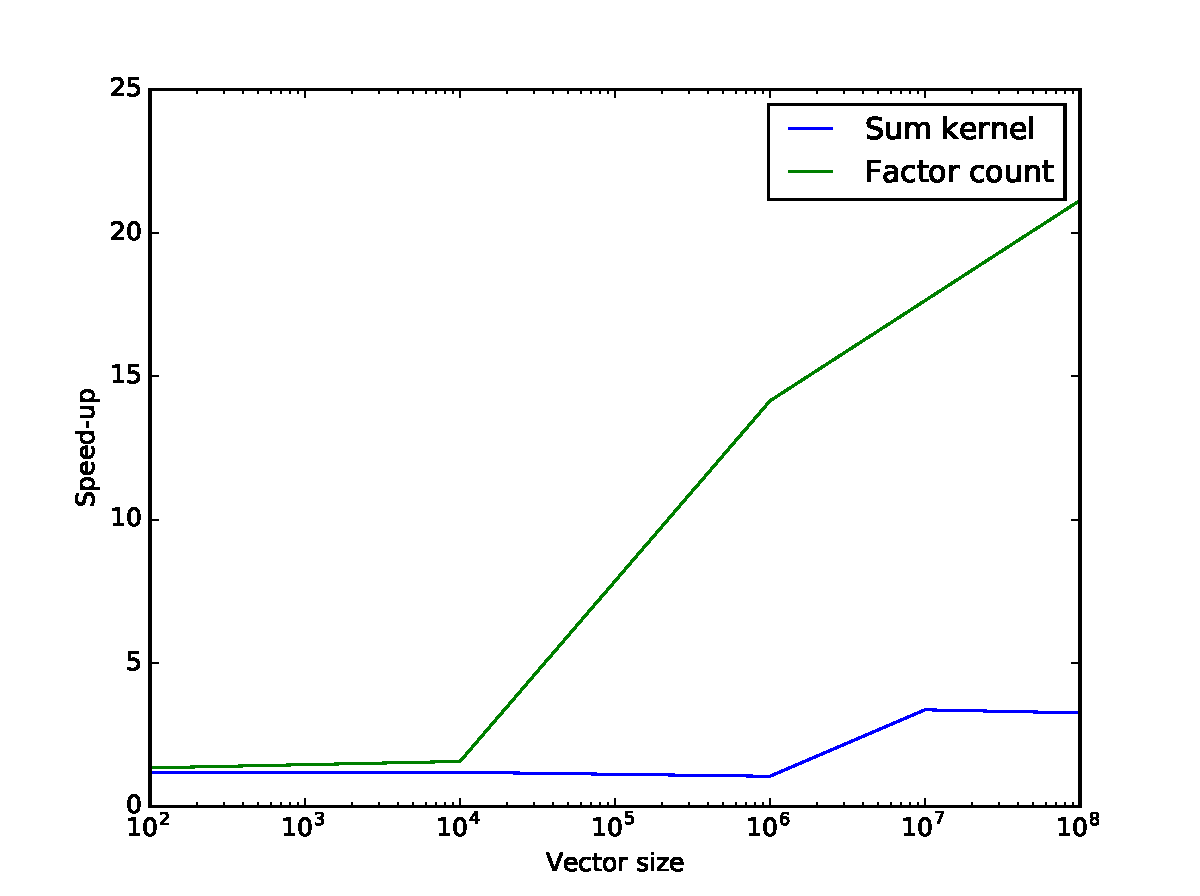
\includegraphics[width=\columnwidth]{Figures/speedup}
\caption{Average speed-up of GPU/CPU vs vector size}
\label{fig:speedup}
\end{figure}


